\chapter{Computo en GPU's}
Hasta hace 12 años la velocidad a la que crecían cada generación de procesadores era increíble, los programas eran tan rápidos como cada nueva generación de procesadores. Este crecimiento entre cada generación se detuvo, el problema es el consumo de energía y la disipación de calor, no permiten aumentar la frecuencia del reloj del procesador y el nivel de actividades por ciclo, en una sola unidad de procesamiento (CPU). Todos los productores de procesadores migraron a un nuevo modelo, los procesadores multinúcleo incrementaron el poder de procesamiento.

Este cambio en los procesadores tuvo un gran impacto a los programadores, la mayoría de las aplicaciones son escritas de forma secuencial,  por que la ejecución de estas son comprensibles paso a paso, mediante el código. Pero un programa secuencial ejecutándose en un solo núcleo del procesador, no sera más rápido. Entonces los programadores ya no pueden agregar cualidades y capacidades a sus programas.

Llega el momento de cambiar, si se desea que la calidad de los programas siga escalando con cada generación de procesadores, se deben crear programas que trabajen con múltiples hilos, cooperando todos para completar un trabajo mas rápido. Existen dos corrientes principales en cuanto a los procesadores multi-núcleo, el primero, es donde se pretende mantener la velocidad de los programas secuenciales, mientras se mueven entre múltiples núcleos; la segunda, se centra mas en la ejecución de aplicaciones en paralelo, tiene un gran numero de núcleos pequeños que va creciendo con cada generación. Es esta rama en la que entran las unidades de procesamiento gráfico o por sus siglas en ingles GPU.\cite{Kirk2010}

\section{GP-GPUs Nvidia}

"Las GPU han evolucionado al punto que muchas aplicaciones del mundo real se están implementando fácilmente en ellas y se ejecutan muchísimo más rápido que en sistemas con múltiples núcleos. Las arquitecturas de computación del futuro serán sistemas híbridos con GPU de núcleos paralelos trabajando en tándem con CPU de múltiples núcleos".\cite{GPUIntro}

\begin{figure}[h]
			\centering
				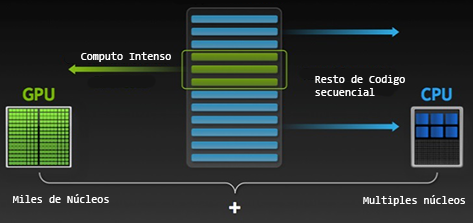
\includegraphics[scale=1]{img/how-gpu-acceleration-works.png}
			\caption{Sistema Híbrido}
\end{figure}

\subsection{Breve Historia}
La necesidad de mejores gráficos para los vídeo juegos, provocaron un gran avance en el hardware que se diseñaría. Desde principios de 1980 hasta finales de 1990 las tarjetas dedicadas a gráficos, no eran más que pipelines fijos que despliegan las formas geométricas calculadas por el CPU, por medio del hardware de acceso directo a memoria, por sus siglas en ingles DMA, esto les daba un funcionamiento fijo y apenas se podía configurar, con principalmente dos API, OpenGL de \textit{Silicon Graphics} y Direct3D de \textit{Microsoft}. Un ejemplo de estas tarjetas gráficas es, a la que se le acuño el nombre de GPU, la GeForce 256\cite{GeForce256} lanzada al mercado en 1999, aporta una capacidad visual sin precedentes, capaz de realizar las funciones de  transformación, iluminación, organización y rendering, con la capacidad de procesar 15 millones de triángulos por segundo y un rendimiento de 480 millones de píxeles por segundo. Su motor de rendering  256 bits muestra una mejora en cuanto a la complejidad visual.

Toda esta tecnología tan revolucionaria llamo la atención de otros profesionales, que se integraron a el trabajo de los artistas y desarrolladores de vídeo juegos, utilizando el gran rendimiento de punto flotante que tenían los GPU para otros objetivos. De esta forma surge el movimiento de la GPU para fines generales(GP-GPU).

Pero en ese momento, la GP-GPU era muy difícil de manipular, solo aquellos que tenían amplios conocimientos en lenguajes de programación de gráficos, desarrollaban para esta plataforma. Pero aun que memorizaras el API entera se enfrentaba un reto, donde los cálculos para resolver problemas generales debían ser representados por triángulos o polígonos.

Fue hasta 2001, en la Universidad de Stanford un equipo, liderado por Ian Buck, que se propuso ver el GPU como un  \textit{procesador de flujos}. Este equipo desarrollaría \textit{Brook} \cite{Buck2001}, un lenguaje de programación diseñado para ser igual a la sintaxis de C, con algunas características adicionales. El lenguaje se desarrolla con el objetivo de minimizar el complejo trabajo de análisis, que se requería para generar aplicaciones paralelas. Introducirían conceptos como los flujos(streams), kernels y los operadores de reducción. Todo esto le dio un gran impulso a los GPU como procesadores de propósitos generales, ya que el lenguaje era mas fácil de manejar, ya que era de más alto nivel, y lo mas importante los programas escritos en \textit{Brook} eran hasta 7 veces mas rápido que códigos similares existentes.

La compañía NVIDIA se dio cuenta que tenia un hardware muy poderoso en las manos, pero debía complementarlo con herramientas de hardware y software intuitivas, con ello le hicieron la invitación a Ian Buck para colaborar con ellos, el objetivo sería ejecutar C a la perfección en una GPU. NVIDIA alcanza este objetivo en 2006 con el lanzamiento de CUDA, la cual seria la primera solución para las GP-GPU, y aunado a esta solución, lanza la GeForce 8800 la cual fue diseñada, para ser usada en cómputo de propósito general, y su arquitectura fue pensada en la de CUDA. 

\section{CUDA}
Compute Unified Device Architecture (CUDA) es una plataforma para computo paralelo y un modelo de programación, que NVIDIA lanzo en noviembre de 2006, permitiendo obtener aumentos en los rendimientos del computo, esto es gracias a la ayuda que la unidad de procesamiento de gráficos, le proporciona al CPU. 

Los dispositivos CUDA aceleran la ejecución de los programas que tienen una gran cantidad de datos a procesar, ya que la arquitectura de esta plataforma, de la cual se hablara adelante, es como un procesador tradicional como el que las computadoras tienen, solo que tienen la cualidad de que los procesadores son masivamente paralelos equipados con una gran cantidad de unidades aritméticas. En las cuales se ejecutara la misma instrucción en todas, respecto a la taxonomía de Flynn, la categoría seria de \textit{una instrucción, multiples datos} (SIMD). 

\begin{figure}[h]
			\centering
				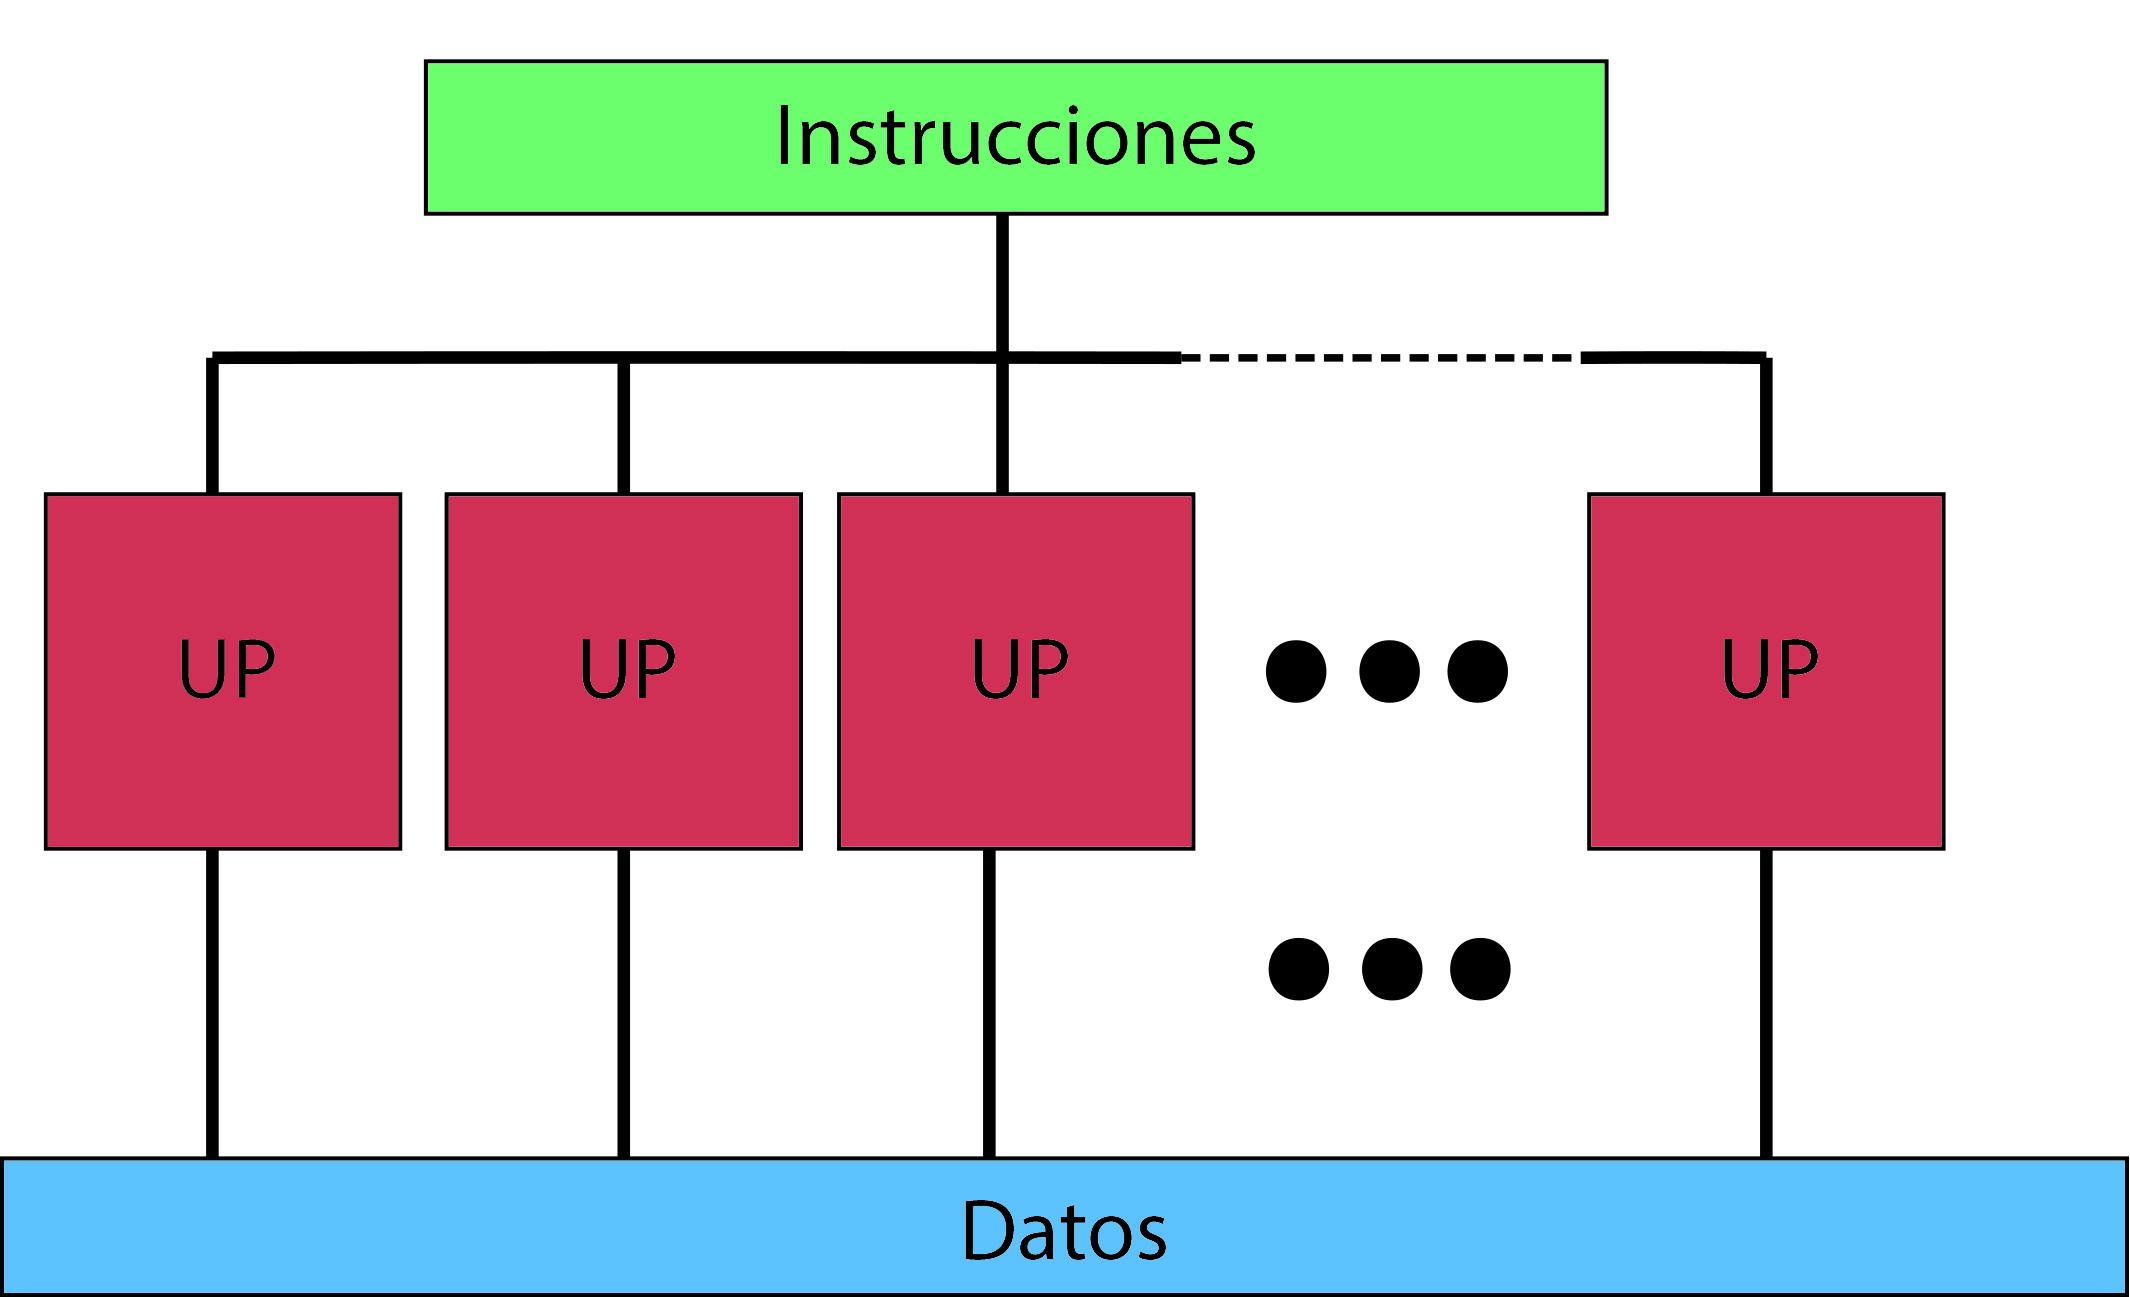
\includegraphics[scale=0.1]{img/SIMD.jpg}
			\caption{SIMD}
\end{figure}


Respecto al modelo de programación para desarrollar los programas para las GPU, es gracias a una extensión del lenguaje C, conocida como CUDA C. Existen alternativas a esta extensión, se pueden utilizar lenguajes como FORTRAN, Python, .NET combinando CUDA con Microsoft's F\# o alguna API como OpenCL u OpenACC\cite{lenguajes}. 
 

\subsection{Arquitecturas}
La arquitectura de CUDA fue diseñada, para que la GPU pudiera ser utilizada en aplicaciones de propósito general. En la cual se tiene un arreglo de procesadores con múltiples unidades aritmético lógica, por sus siglas en ingles ALU, las cuales para alcanzar este objetivo, fueron diseñadas para poder realizar operaciones de punto flotante, cumpliendo los requisitos del Instituto de Ingeniería Eléctrica y Electrónica (IEEE). Aparte de esto las ALU debían tener acceso a diferentes tipos de memoria, como la compartida entre unidades y la memoria de la tarjeta gráfica. 

Estas ALU tan particulares, en la arquitectura de CUDA las conoceremos como \textit{CUDA cores}, conforman gran parte de los Streaming Multiprocessor (SM). Los SM son procesadores que tienen la tarea de ejecutar los hilos concurrentemente, aparte de los CUDA cores tienen, están formados por una memoria cache(shared memory), registros y algunas unidades de funciones especiales.

\subsubsection{Fermi}

Los GPU basados en la arquitectura Fermi \cite{fermi}, están formados por 512 CUDA cores. Los CUDA cores ejecutan operaciones de punto flotantes o enteras por ciclo de reloj, y por cada uno de los hilos. Los 512 CUDA cores están organizados en 16 SM de 32 cores cada uno. El GPU tiene seis particiones de memoria de 64-bits, capacidad para leer 384-bits de la memoria simultáneamente y con una capacidad de hasta 6GB de memoria DRAM categoría DDR5. El sistema de conexión entre el GPU y el CPU es vía PCI-Express. La forma en que se hace la programación de el trabajo a realizar en cada bloque es asignado por un modulo llamado \textit{GigaThread}, este pasa las tareas a cada SM para que el haga la asignación de trabajo a cada hilo. 

\begin{figure}[h]
			\centering
				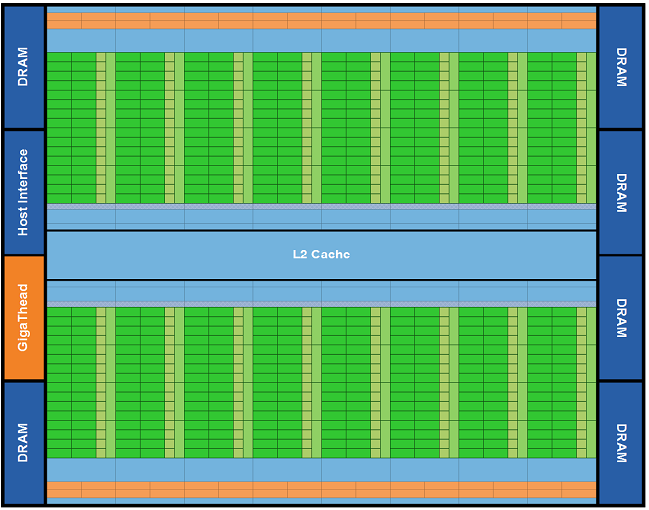
\includegraphics[scale=0.7]{img/ArqFermi.png}
			\caption{La arquitectura Fermi tiene sus 16 SM al rededor de la memoria compartida L2 cache}
\end{figure}

La arquitectura tuvo mejoras significativas como el rendimiento en las operaciones de doble precisión, dedicado a computo científico; soporte para la corrección de errores, para asegurar las operaciones con números muy grandes, en aplicaciones delicadas; se implemento una jerarquía en la memoria cache, que permite aumentar la eficiencia en cuanto a las  lecturas a memoria; la memoria compartida tuvo un incremento; y las operaciones atómicas incrementaron su desempeño, gracias a que se aumentaron las unidades de operaciones atómicas y la aparición de la memoria L2 cache. 

\begin{figure}[h]
			\centering
				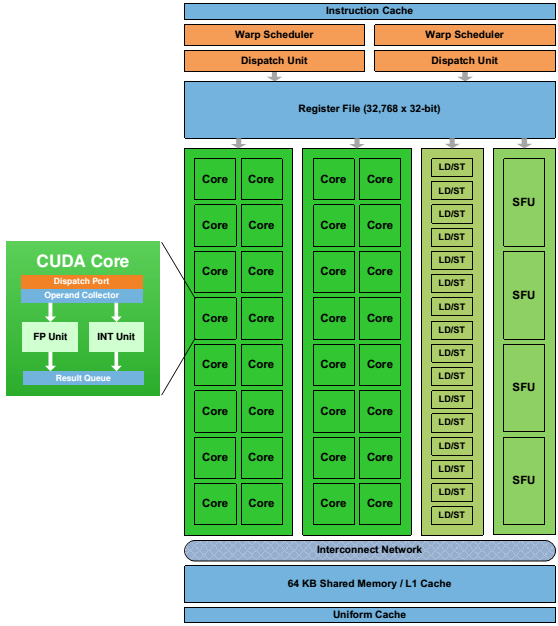
\includegraphics[scale=0.6]{img/fermiSM.png}
			\caption{Fermi Streaming Multiprocessor (SM)}
\end{figure}

Las SM de la arquitectura Fermi están formadas de diferentes elementos, iniciando por los 32 CUDA cores, cada uno con una unidad aritmética lógica para las operaciones con enteros y una unidad de punto flotante. Cumplen con la norma IEEE 754-2008 que permite realizar una multiplicación y una suma en un solo paso de redondeo. La asignación de trabajo en las SM se realiza por el modulo \textit{GigaThread}, que divide en bloques de hilos a cada SM, después los planeadores de \textit{warps} es quien tienen el trabajo de dividir este bloque en grupos de 32 hilos para su ejecución dentro de la SM. Tambien tiene 16 unidades load/store, las cuales permiten calcular origen y destino de dieciséis hilos por pulso de reloj; cuenta también con 4 unidades de funciones especiales (SFU), que ejecutan instrucciones mas complejas como senos, cosenos, reciproco y raíz cuadrada. 

\subsubsection{Kepler}

La arquitectura Kepler \cite{Kepler}, modifico los SM de su antecesor llamándolo Next Generation Streaming Multiprocessor (SMX), es el nuevo procesador de esta arquitectura, en la cual encontraremos que esta formada por 15 de estos procesadores y seis controladores de memoria de 64-bits.La cantidad de CUDA cores que contiene es de 192 de precisión simple y 64 unidades de doble precisión. 

Las unidades load/store aumentaron a 32 y las SFU también incrementaron a 32, ocho veces más que en Fermi. La asignación de hilos dentro de el SMX es programado igualmente por planeadores de warps, bloques de 32 hilos, Kepler tiene 4 planificadores de warps, de esta manera se tienen 2 unidades de despacho de instrucciones, permitiendo repartir y ejecutar 4 warps de manera concurrente. Nos encontramos con una memoria cache L1, la cual podemos cambiar su configuración. 

\begin{figure}[h]
			\centering
				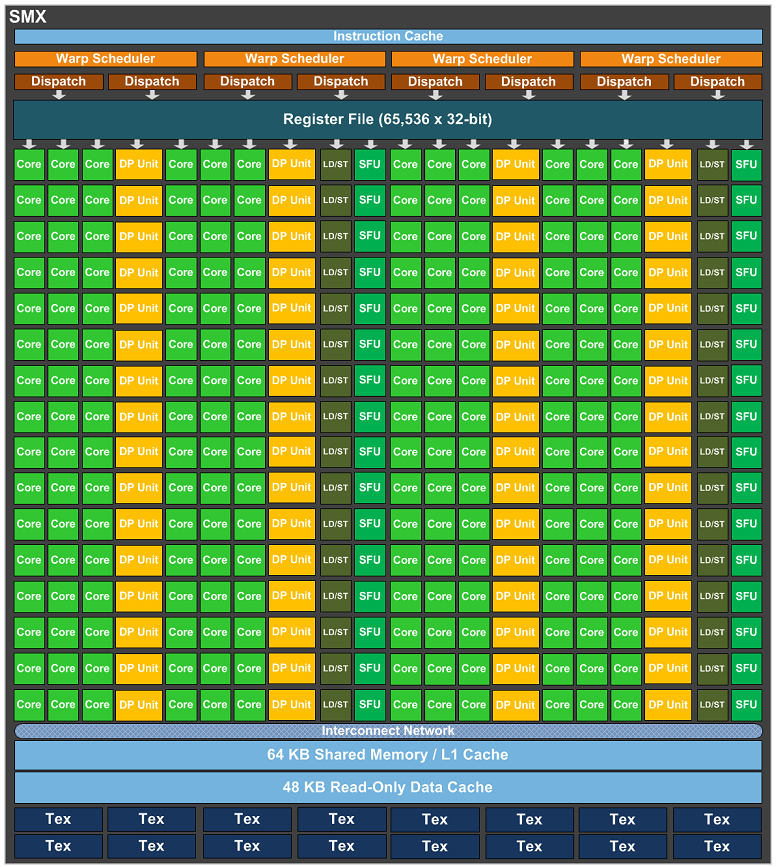
\includegraphics[scale=0.4]{img/KeplerSMX.png}
			\caption{Kepler Next Generation Streaming Multiprocessor (SMX)}
\end{figure}

La capacidad de esta memoria es de 64KB, se pueden tener las configuraciones de 16, 32 o 48 KB para la memoria cache, dejando el resto para la memoria compartida. La cantidad de registros por SMX es de 65536, de los cuales, cada hilo puede tener acceso a 255 registros para el almacenamiento de datos. La memoria de textura ha sido un recurso valioso para para programas donde se requiere probar o filtrar datos de una imagen, en esta arquitectura dejo de ser un hardware dedicado solo a este objetivo, se dejo un espacio en la memoria global de solo lectura de 48KB que funciona como una memoria cache para agilizar las lecturas.



En esta arquitectura se agrego una característica, donde no se requiere de el CPU para lanzar programas en la GPU, lo que significa que el GPU tiene la capacidad de generar mas carga de trabajo, administrar recursos y obtener resultados dentro de la misma GPU, en la zona de mas interés, donde se pueda requerir más poder de computo. 

\begin{figure}[h]
			\centering
				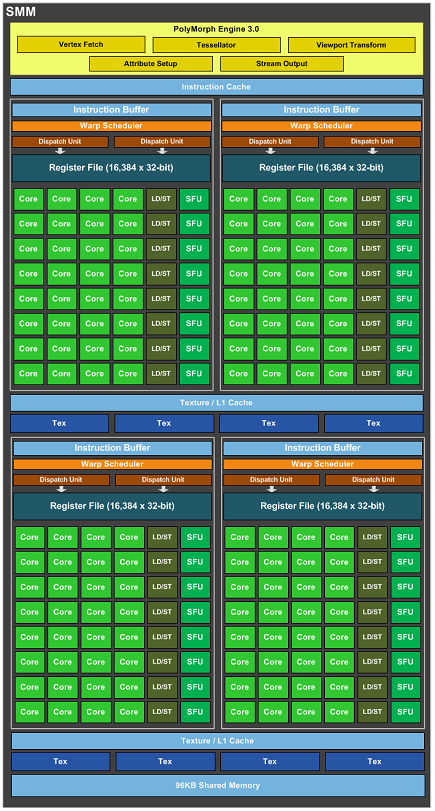
\includegraphics[scale=0.45]{img/MaxwellSM.png}
			\caption{Maxwell Streaming Multiprocessor (SMM)}
\end{figure}



\subsubsection{Maxwell}
La arquitectura Maxwell\cite{Maxwell}, tuvo un cambio en su diseño para proporcionar un cambio dramático en su desempeño. Lo que genero este desempeño fue el nuevo diseño que le dieron a los nuevos SM llamados SM Maxwell (SMM). El numero de CUDA cores bajo a 128, para poder separarlos en 4 divisiones de 32 CUDA cores, cada una de esas divisiones tiene un planificador de warps, para su bloque de 32 CUDA cores, el cual es capaz de despachar dos instrucciones por ciclo de reloj. Estas divisiones hicieron que se utilizara de una manera mas eficiente el espacio y la energia gastada para el manejo de la transferencia de datos.

La memoria compartida incremento a 96KB, la cual ya no se comparte con la memoria cache L1, ahora la memoria de textura comparte espacio con la cahce L1. Los registros, las SFU, y las unidades load/store siguen siendo la misma cantidad.



\section{Modelo de Programación CUDA C}
La extensión del lenguaje C que proporciona CUDA para programar, es un camino que ofrece, para programadores familiarizados a este lenguaje, una manera sencilla de escribir programas para ser ejecutados en la GPU. A continuación se explicara el núcleo del conjunto de instrucciones de esta extensión.
\subsection{Kernels}

En CUDA C, permite definir funciones llamadas \textit{kernels}, las cuales cuando son llamadas se ejecutan N veces en paralelo por N diferentes \textit{hilos} CUDA. Para definir un kernel se usa la declaración \textbf{\_\_global\_\_}, estos kernels se ejecutan en un dispositivo, la tarjeta gráfica instalada en la computadora; y se invocaran por medio de un equipo anfitrión, este anfitrión no es mas que el procesador que estará usando la tarjeta gráfica como coprocesador. En el siguiente código podemos ver como se declara un kernel: 

\lstset{language=C,
                basicstyle=\ttfamily,
                keywordstyle=\color{blue}\ttfamily,
                stringstyle=\color{red}\ttfamily,
                commentstyle=\color{green}\ttfamily,
        frame= single,
        numbers = left,
        xleftmargin=2em,
        framexleftmargin=1.5em        
}
\begin{lstlisting}
	__global__ void kernel( ... )
    {
   		...
    }

\end{lstlisting}

Al lanzar, desde el anfitrión, el kernel, se debe escoger una configuración de hilos CUDA que se lanzaran para ejecutarlo, a cada uno de estos hilos se les dará un identificador único (\textit{threadID}). 

\subsection{Jerarquía de Hilos}

Para especificar la configuración que se usara para lanzar los hilos, se especifica poniéndolo entre \textbf{\textless\textless\textless} y \textbf{\textgreater\textgreater\textgreater}.Se requiere de dos parámetros para el lanzamiento el primero es la dimension de la malla, que se refiere al numero de bloques y el segundo es la dimension del bloque, que es el numero de hilos que contendrá. 


\begin{figure}[h]
			\centering
				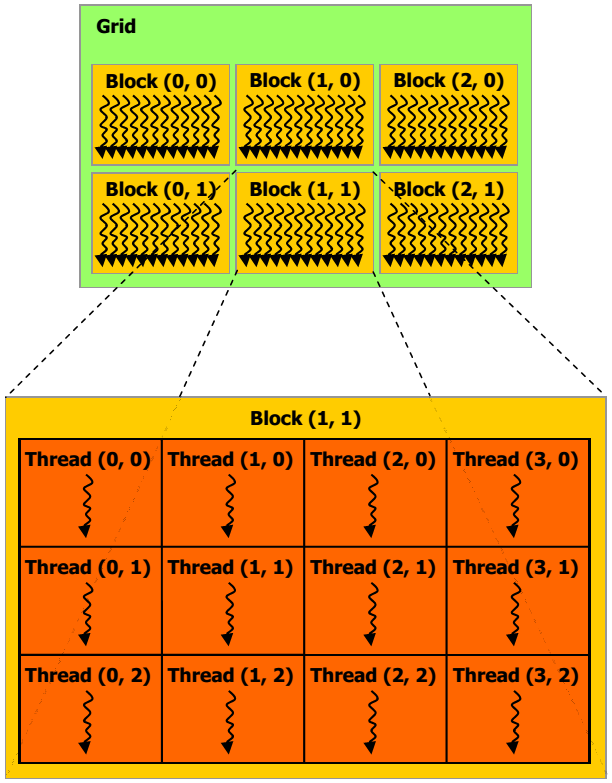
\includegraphics[scale=0.45]{img/grid_block.png}
			\caption{Organización de bloques e hilos}
\end{figure}


Cada hilo tiene un identificador que se puede acceder por \textbf{threadIdx}, este identificador es un vector de tres componentes, por lo tanto los hilos pueden usar identificadores de uno, dos o tres dimensiones. Para formar bloques unidimensionales, dimensionales o tridimensionales. Los bloques están organizados en una malla que puede tener una, dos o tres dimensiones, los bloques tiene un identificador al cual se puede acceder por la variable \textbf{blockIdx}, existe otra variable importante y es la que nos dará la dimension del bloque, se llama \textbf{blockDim}. A continuación veremos un ejemplo de como se lanzaría un kernel:

\lstset{language=C,
                basicstyle=\ttfamily,
                keywordstyle=\color{blue}\ttfamily,
                stringstyle=\color{red}\ttfamily,
                commentstyle=\color{green}\ttfamily,
        frame= single,
        numbers = left,
        xleftmargin=2em,
        framexleftmargin=1.5em        
}
\begin{lstlisting}
	__global__ void miKernel( ... )
    {
   		...
    }
	int main(...)
	{
		...	
		dim3 gridDim(...,...,...);
		dim3 blockDim(...,...,...);
		miKernel<<<gridDim,blockDim>>>(...);	
		...
	}
\end{lstlisting}

\begin{figure}[h]
			\centering
				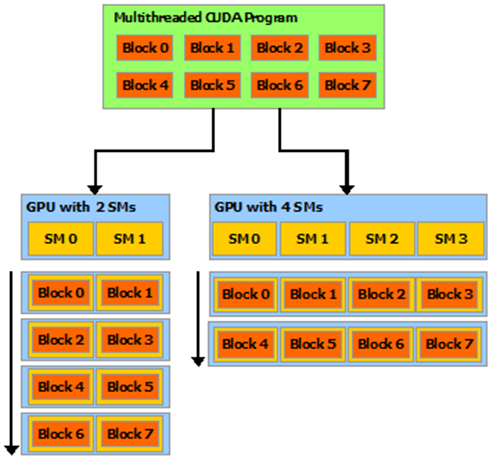
\includegraphics[scale=0.4]{img/block_sm.png}
			\caption{Asignación de bloques por SM}
\end{figure}


Parte importante del paralelismo es la comunicación entre cada proceso que se ejecuta simultáneamente, hacer cooperar los hilos en la GPU tiene sus detalles. Para la comunicación tenemos la memoria compartida a la cual permite el intercambio de datos solo entre hilos del mismo bloque. En cuanto a sincronizar los hilos se tiene una función llamada \textbf{\_\_syncthreads()}, esta sincroniza los hilos por barrera, pero los hilos que esperaran solo lo harán con hilos de su mismo bloque. Esta característica de que solo hilos del mismo bloque se puedan comunicar es por la forma en que son asignados para su ejecución cada uno de los bloques. En la figura 3-8 podemos observar como se asignan los bloques a cada SM por lo tanto podrían asignarse en cualquier orden y ejecutarse en tiempos diferentes. De este modo la sincronizar los hilos y la escritura y lectura a memoria compartida no serán un problema con el diseño que se describió anteriormente.




\subsection{Jerarquía de Memoria}


Los hilos de un kernel son los encargados de realizar las operaciones sobre los datos, se tiene diferentes tipos de almacenamientos en la arquitectura CUDA de los cuales se pueden leer los datos para operar y escribir los resultados obtenidos. Cada uno de estos almacenamientos tiene características diferentes, que nos ayudaran a mejorar el despeño de los programas. A continuación hablaremos de los tipos de memoria que se encuentran en las GPU de Nvidia.

\begin{figure}[h]
			\centering
				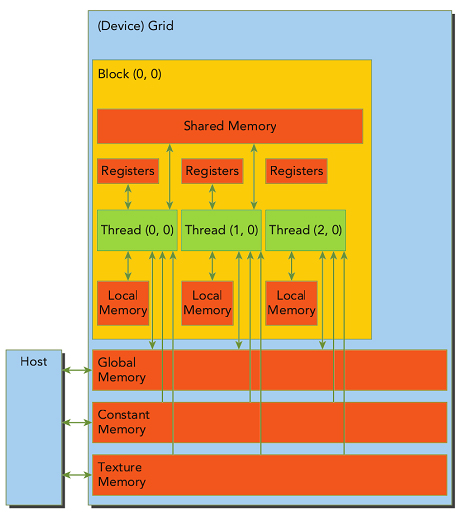
\includegraphics[scale=0.6]{img/memoria.jpg}
			\caption{Tipos de Memoria}
\end{figure}

Los \textit{registros} son el tipo de memoria con la lectura/escritura mas rápida que ninguna otra en el dispositivo. En cada SM tenemos miles de registros y a cada hilo se les asigna una cantidad de estos registros, cuando es lanzado el kernel. Los registros son de 32-bits en los cuales se pueden almacenar datos de tipo flotante o entero. La manipulación de este espacio esta administrado por el sistema.

La \textit{memoria local} es un espacio de memoria privada que cada hilo tiene, podemos ver que se almacenan datos que no pudieron ser almacenados en los registros como variables locales, llamadas a funciones y el contexto de ejecución. Al igual que los registros esta memoria es administrada por el sistema.

La \textit{memoria compartida} es una memoria de tipo cache que se comparte entre hilos de un mismo bloque, esto genera que los hilos de el bloque puedan comunicarse, escribiendo y leyendo en ella, para cooperar en la realización de un mismo objetivo. Este cache es especial ya que el programador elige su manejo, la forma en la que se declara una variable en este espacio, es con ayuda de la palabra reservada \textbf{\_\_shared\_\_}. La latencia en esta memoria es hasta 100 veces menor en comparación con la memoria global. 

La\textit{ memoria constante} es una memoria de solo lectura, en la cual albergaremos datos que no cambiaran a lo lago de la ejecución del kernel. Podemos ubicar esta memoria en el dispositivo, al igual que la memoria global, pero esta esta optimizada para enviar datos de lecturas a múltiples hilos. Esto se logra gracias a diferentes instrucciones  que permiten el acceso a este cache de una forma mas eficiente. Con la palabra reservada \textbf{\_\_constant\_\_}, se puede declarar la variable, pero el contenido de este debe ser asignado por el anfitrión, en la memoria del dispositivo, antes de lanzar el kernel, con ayuda de la función \textbf{cudaMemcpyToSymbol()}.

La \textit{memoria de textura} al igual que la memoria constante es una memoria de solo lectura, esta diseñada para trabajar con estructuras llamadas CUDA array las cuales permiten un lecturas eficientes en arreglos de una, dos o tres dimensiones. Las lecturas en este tipo de memoria tienen ventajas como diferentes formas de acceso e interpolaciones en los datos que se pueden utilizar sin costos adicionales.




La \textit{memoria global} es la memoria de lectura/escritura de mayor tamaño en la tarjeta gráfica, llega al orden de los gygabytes. Las funciones que tiene son de lectura de datos y escritura de resultados, también funciona como interfaz entre la GPU y el CPU. La persistencia de los datos en esta memoria son persistentes, hasta que se liberen, lo que nos permite que esta memoria funcione para compartir datos entre kernels. Los hilos pueden acceder en cualquier momento del kernel a esta memoria, pero su latencia es tan alta que podría provocar que tarde mas la lectura de datos que los cálculos que se quieren realizar. Existen funciones para reservar, manejar y liberar el espacio en memoria, desde el anfitrión: \textbf{cudaMalloc()}, \textbf{cudaMemCpy()} y \textbf{cudaFree()}.



\subsection{Programación heterogénea}

\begin{figure}[h]
			\centering
				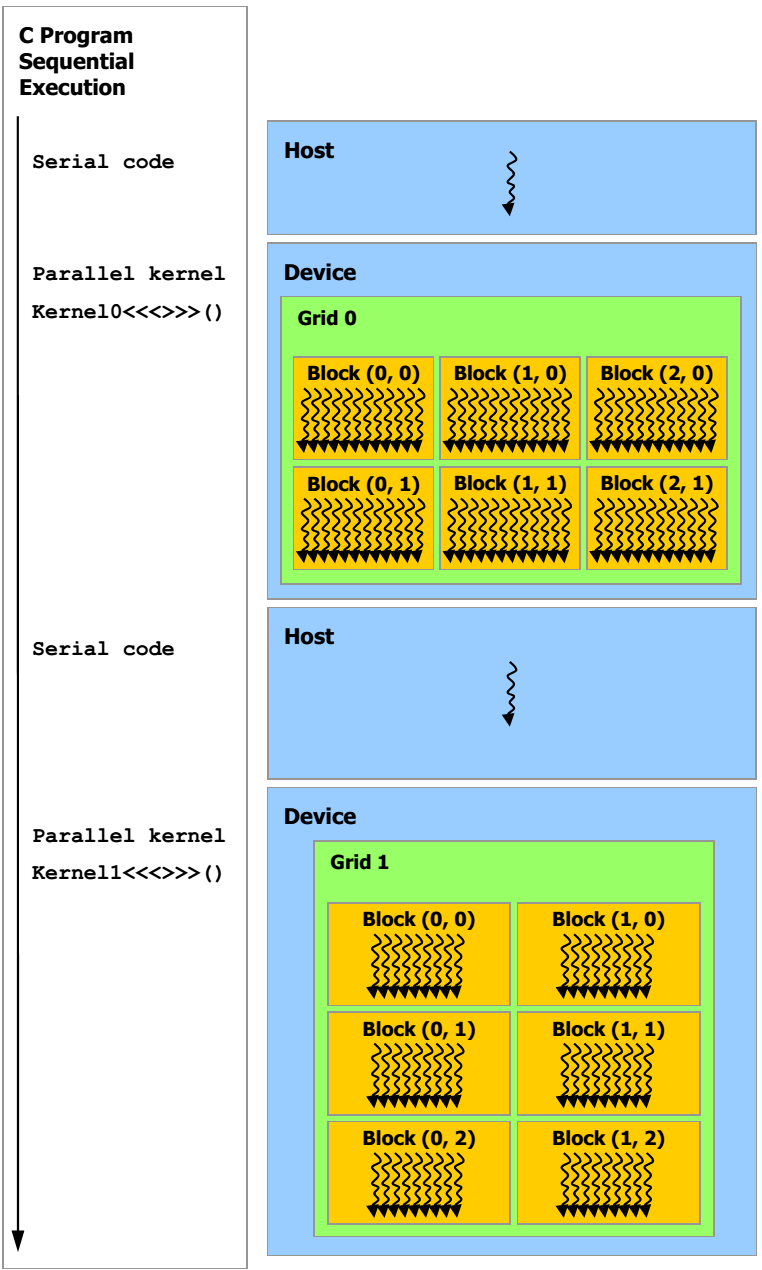
\includegraphics[scale=0.35]{img/PH.png}
			\caption{Programación Heterogénea}
\end{figure}

Para entender el modelo de programación de CUDA, se tiene que tener en cuenta que se debe hacer código para el CPU y el GPU para que estos puedan trabajar en conjunto. El CPU es el equipo anfitrión (Host) el que decidirá cuando necesitara usar al dispositivo (Device) GPU, el anfitrion y el dispositivo también tendrán memorias separadas. 

Un Programa en CUDA C se ejecuta como se muestra en la figura 3-10, en el siguiente código se puede ver la estructura básica de un programa, en el cual podemos ver que se declara y definen funciones kernel, también podemos ver que hay funciones ejecutables en el GPU, siendo llamadas desde algún kernel se definiran con la palabra reservada \textbf{\_\_device\_\_}.
En la función principal el anfitrión se encargara de obtener los datos que se le proporcionaran y almacenarlos al kernel para ser procesados por el  GPU, también podemos ver como es que se reservara la memoria en el dispositivo para los datos de entrada y salida que el kernel necesite para procesarlos.
Después de realizar la copia de los datos de anfitrión a dispositivo, se pueden ejecutar uno o más kernels en el GPU, una vez finalizada la ejecución de estos kernels el resultado se copia a la memoria del anfitrión. La final solo quedan liberar los recurso que ya no serán utilizados. 

\lstset{language=C,
                basicstyle=\ttfamily,
                keywordstyle=\color{blue}\ttfamily,
                stringstyle=\color{red}\ttfamily,
                commentstyle=\color{green}\ttfamily,
        frame= single,
        numbers = left,
        xleftmargin=2em,
        framexleftmargin=1.5em        
}
\begin{lstlisting}
	__device__ L funcionDevice()
	{ ... }	
	__global__ void KernelUno(L*, ... )
    {
    	...
   		L r= fooDevice();
   		...
    }
    __global__ void KernelDos( ... )
    { ... }    
    int main(...)
	{	...
		L* datosD;
		cudaMalloc(&datosD,size);
		...		
		cudaMemcpy(datosD,src,size,cudaMemcpyHostToDevice);		
		...	
		dim3 gridDim(...,...,...);
		dim3 blockDim(...,...,...);
		KernelUno<<<gridDim,blockDim>>>(datosD,...);	
		...
		KernelDos<<<...,...>>>(...);
		...
		cudaMemcpy(res,datosD,size,cudaMemcpyHostToDevice);
		...
		cudaFree(datosD);
		...			
	}
\end{lstlisting}




  





\section{Rendimiento}

